\chapter{Apache Spark and Spark Streaming}
\label{spark}

\section{Introduction}
\label{sp:intro}

Apache Spark~\cite{spark} is a general purpose data processing framework that supports wide range of applications from \emph{batch} processing, \emph{stream} processing, \emph{graph} processing to \emph{machine learning}, etc. In this chapter the architecture of Apache Spark and Spark Streaming -- as one of its sub projects -- will be explored and discussed. Throughout the chapter, minor examples will also be presented to further simplify the concepts. This chapter is organized as follows. Section~\ref{sp:basics} explains the basic concepts of Apache Spark. Then, section~\ref{sp:rdd} explains \emph{Resilient Distributed Datasets} (RDDs) which is the most integral component of the Apache Spark. Section~\ref{sp:dstream} explains \emph{Discretized Streams} (DStreams) as the fundamental building block for data stream processing applications. Finally, section~\ref{sp:conc} concludes this chapter.

\section{Basic Concepts}
\label{sp:basics}

Map-Reduce~\cite{Dean:2004} and its derivative projects have been widely used by \emph{data-oriented} applications to process and crunch huge datasets over last the decade. In traditional Map-Reduce environments, developers typically create \emph{acyclic} data flow graphs to process input data. However, as confirmed by \textcite{Zaharia:2010}, there are two categories of applications that are not well suited for this architecture.
\begin{itemize}
    \item \textbf{Iterative Jobs} Many machine learning applications process the same input \emph{iteratively}. In traditional model, each iteration should be defined as a separate MapReduce job. While this is feasible, but for each job, input data has to be loaded from disk which leads to serious performance issues.
    \item \textbf{Interactive Analysis} MapReduce derivative projects like Hive~\cite{hive} and Pig~\cite{pig} have been extensively used to run SQL queries on top of massive datasets. Whenever a user submits different queries over the same dataset, the ideal solution would be to load all datasets into memory once and then execute different queries on top of it. However, with traditional model of execution each query shall be defined as a separate job which reads input data from disk.
\end{itemize}
Apache spark has been designed from ground up to resolve these issues. It provides a large stack of tools to facilitate processing large datasets. Figure~\ref{fig:spark-eco} depicts tools provided by Spark.
\begin{figure}[h]
    \centering
    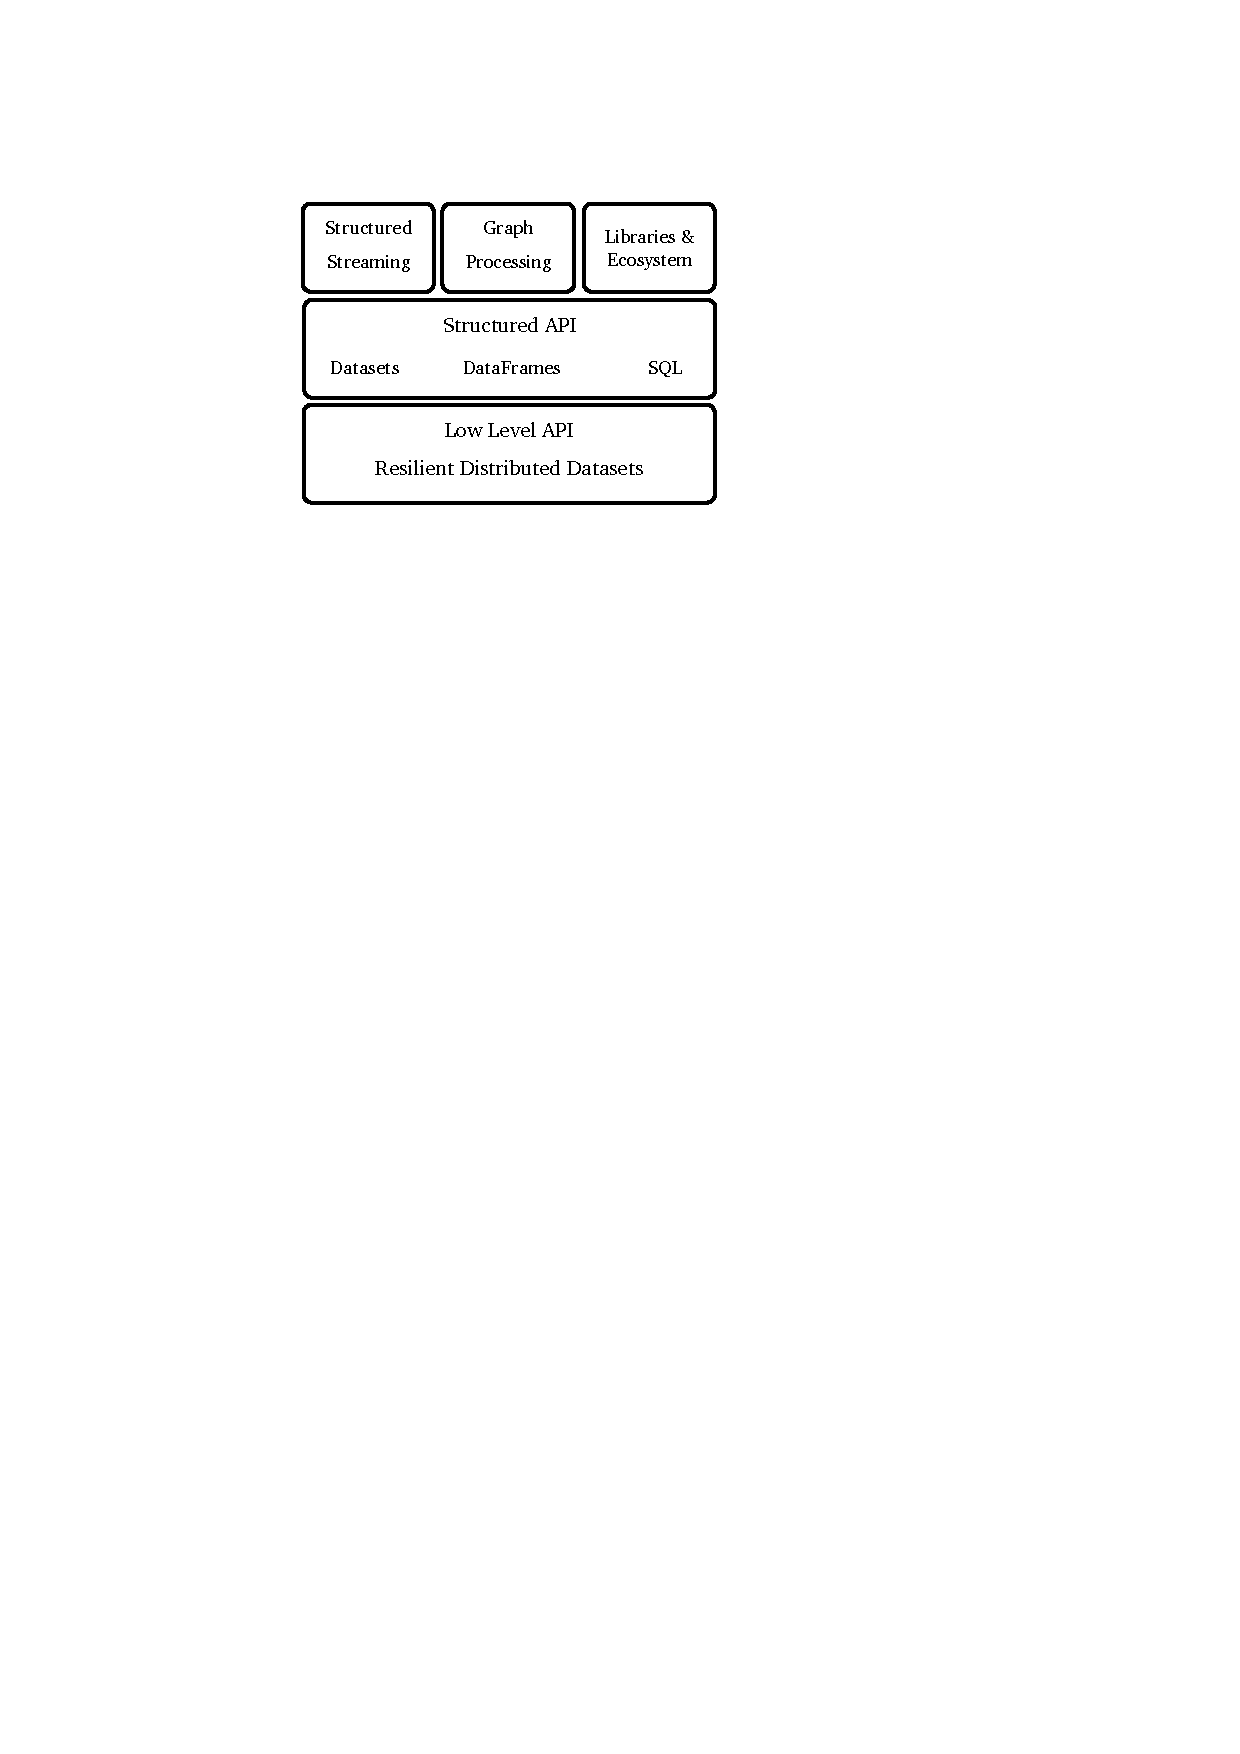
\includegraphics[clip,trim=5cm 21.2cm 8.7cm 3.4cm]{spark-eco.pdf}
    \caption{Apache Spark Stack}
    \label{fig:spark-eco}
\end{figure}

\subsection{Spark Runtime Architecture}
\label{sp:run}

Any Spark application consists of multiple components at runtime. The following lists the relevant components from a high level point of view.
\begin{description}[leftmargin=0pt]
    \item[Driver Process Driver] It is the core component of every Spark application. It is a single process and runs on one of the nodes in the cluster. It maintains all the critical information such as user's program, input files, output files and data flow of the application. The driver process should run during the runtime the of the application. In case driver process fails, the whole application is considered as \emph{dead} and should be restarted by any \emph{fault-tolerant} mechanism available in the cluster.
    \item[Distributed File System] It provides a shared file system accessible by any node in the cluster. There is no limitation on type of the file system but typically \emph{Hadoop Distributed File System} (HDFS)~\cite{hadoop} is used.
    \item[Worker Processes] A collection of worker processes known as \emph{executors} that run on cluster nodes. Executors run user defined code. During the runtime of the application each worker consume any number of input records, processes it based on user defined code and emits any number of output records. Similar to driver process, liveness of the worker processes shall by monitored. However, the role of worker processes are not as critical as driver process, even though they may fail for any reason. Workers have access to load/store data files from/to distributed file system or local memory of the machine. During lifetime of the application, status of the workers will be reported to driver process.
    \item[User Defined Code] Provided by user and caries the main logic of the application.
\end{description}
Figure~\ref{fig:spark-runtime} depicts coarse grained architecture of a Spark application and table~\ref{tab:spark-runtime} summarizes these components.
\begin{figure}[h]
    \centering
    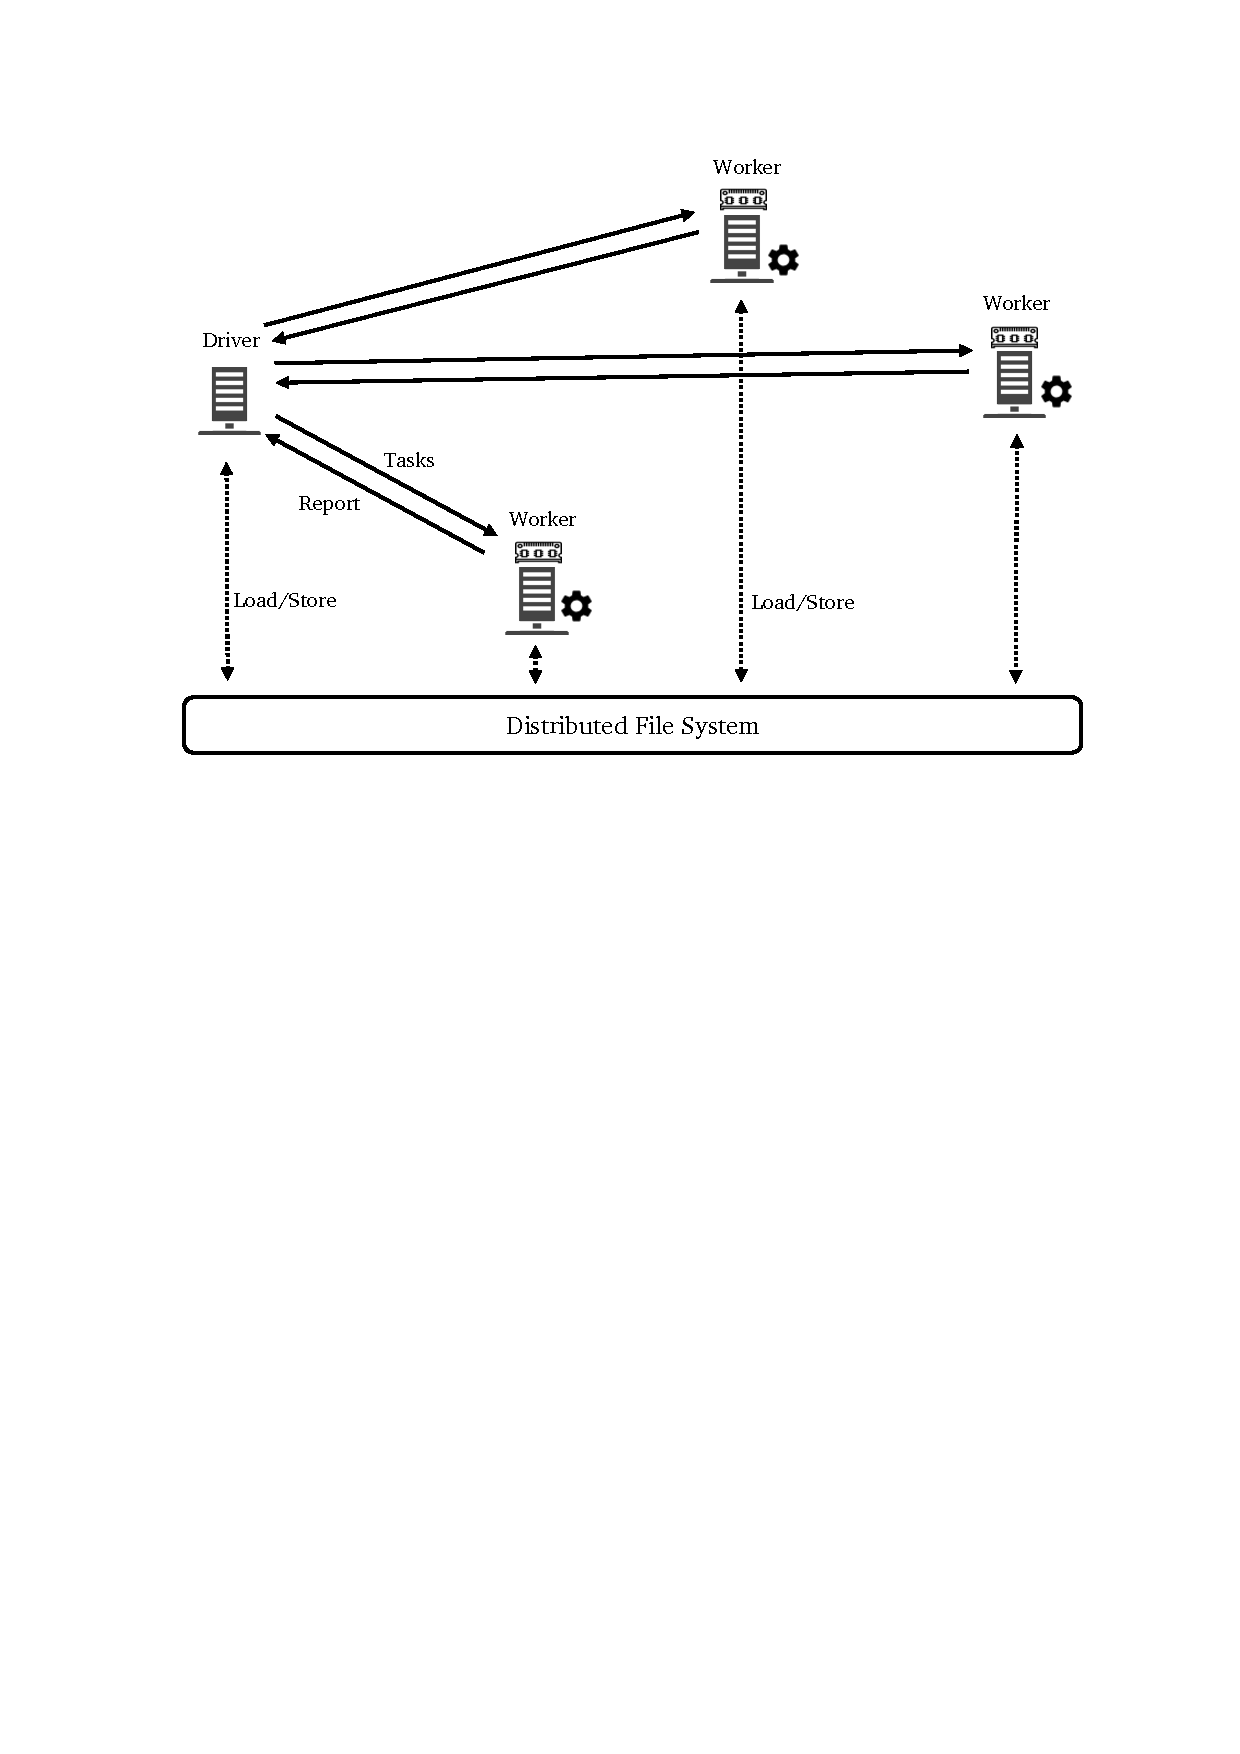
\includegraphics[clip,trim=3cm 16.8cm 2.5cm 2.5cm]{spark-high.pdf}
    \caption[Spark Runtime Architecture]{Spark Runtime Architecture\footnotemark}
    \label{fig:spark-runtime}
\end{figure}
\footnotetext{The figure has been partially taken from~\cite{Zaharia:2012}}
\begin{table*}[ht]
    \begin{tabularx}{\textwidth}{lX}
        \toprule
        \textbf{Component} & \textbf{Description}\\
        \midrule
        Driver & Maintains all relevant information -- including user defined code -- to process input data and produce output.\\
        Distributed File System & Provides shared file system accessible by all nodes in cluster.\\
        Worker Process & Workforce of the cluster. Gets necessary information from driver and executes user defined code.\\
        User Defined Code & Caries the main application logic.\\
        \bottomrule
    \end{tabularx}
    \centering
    \caption{Summary of Spark runtime components}
    \label{tab:spark-runtime}
\end{table*}

\subsection{Spark Cluster Manager}
\label{sp:cluster}

Section~\ref{sp:run} described the coarse grained architecture of Spark. However, from a more fine grained point of view, there is missing component known as \emph{Cluster Manager}. Cluster Manager controls the \emph{assignment} of executors to cluster nodes. It monitors liveness of executors during lifetime of the Spark application. \emph{Spark Session} has the responsibility to communicate with Cluster Manager and executors.
\begin{figure}[h]
    \centering
    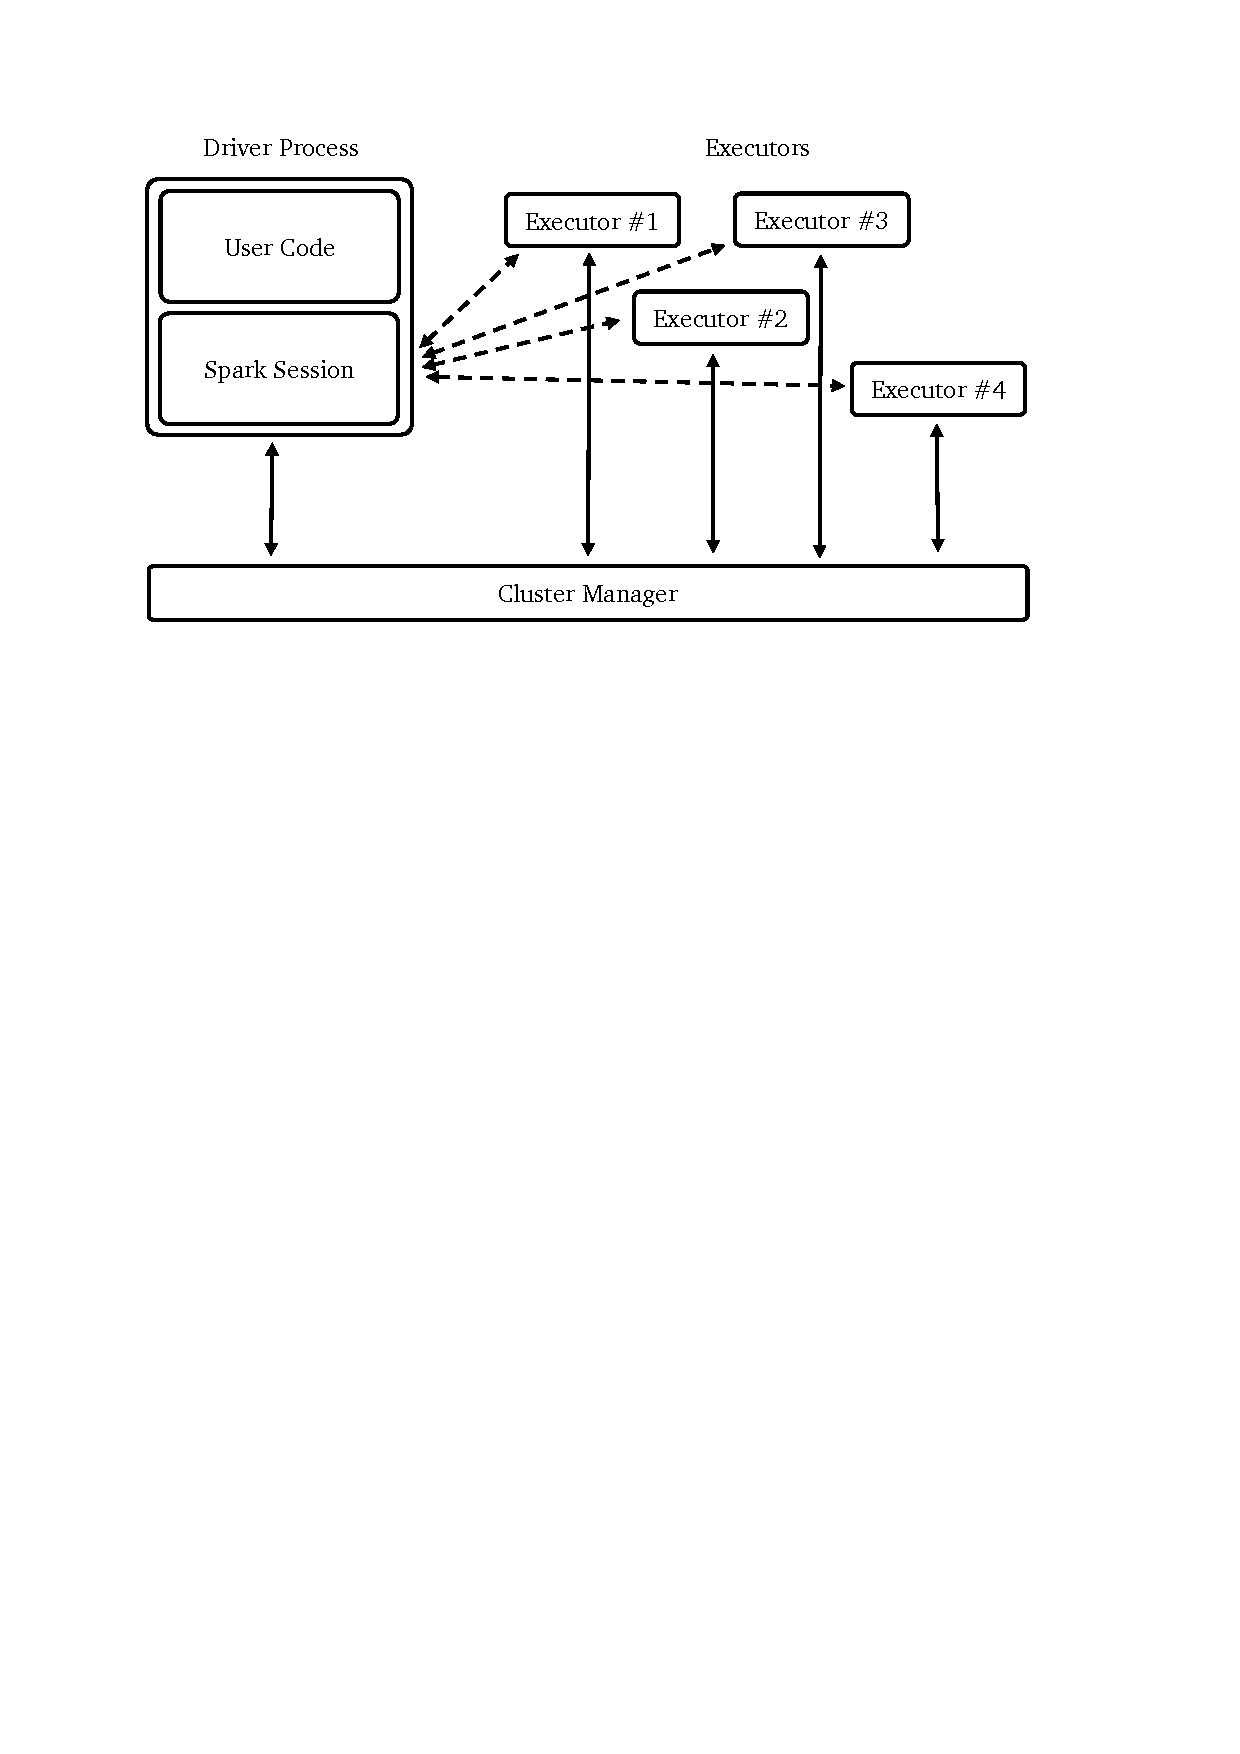
\includegraphics[clip,trim=2.4cm 19cm 3.5cm 2cm]{spark-cluster.pdf}
    \caption[Spark Cluster Manager Architecture]{Spark Cluster Manager Architecture\footnotemark}
    \label{fig:spark-cluster}
\end{figure}
\footnotetext{The figure has been partially taken from~\cite{spark-guide}}

Note that, the term \emph{executor} is a conceptual term and implementation details may differ among different resource managers. Spark supports multiple Cluster Manager implementations. The following describes the most prominent implementations. It shall be noted that this list is a growing over time due to Spark's pluggable resource manager architecture.
\begin{description}[leftmargin=0pt]
    \item [Apache YARN] It is referred as \emph{Yet Another Resource Negotiator}~\cite{Vavilapalli:2013} and is the default resource manager for modern Hadoop workloads. It has a master-slave architecture and consists of a single global \emph{Resource Manager} -- most probably accompanied by a backup as well --  and several \emph{Node Managers} that run on each worker node. The concept of executor is implemented as \emph{containers} in YARN. Each container can hold a specific amount of node's processing power (CPU, RAM, Network, etc.). In YARN, any application is modeled with two components. First, \emph{Application Master} that maintains the necessary information to run the application -- Spark driver process in this case and second, several \emph{Workers} that run the user defined code. Both Application Master and Workers are executed in the context of YARN containers. 
    
    Fault-tolerance is provided at multiple levels. First, several backup nodes monitor the master resource manager via Zookeeper. In case master resource manager fails, one of the backup masters takes over the responsibility. Second, Applications Master reports its status to the global resource manager. In case, application master fails, the global resource manager launches a new Application Master on another node. Third, Workers provide different progress reports to Application Master and Node Managers. In case any Worker container fails, a new container will be allocated and the old one will be killed by the local Node Manager.
    \item [Apache Mesos] It is another dominant cluster scheduler for Spark~\cite{Hindman:2011}. It is a master-slave resource manager. A global resource manager -- known as \emph{Mesos Master} -- has cluster level view. On each node runs a single \emph{Mesos Slave} process. Mesos has a pluggable architecture for different class of application schedulers. That is, a single cluster can run a mixture of Spark, MPI, etc. jobs with different prioritizes for each application type. Each \emph{Framework Scheduler} handles corresponding jobs. For example, Spark scheduler, maintains multiple driver processes or MPI scheduler maintains multiple MPI applications. Free resources on each Mesos Slave are represented as empty \emph{slots} -- very much like containers in YARN -- and are allocated to one of the currently running jobs.
    
    Fault-tolerance is provided by a similar hierarchical approach like YARN. Mesos Master is monitored by several backups through Zookeeper. Mesos Slaves as well as Framework Schedulers are in turn monitored by Mesos Master. Each job is further monitored by corresponding Framework Scheduler. And finally, executors are monitored by Mesos Slaves. 
    \item [Spark Standalone] It is the default resource manager for Spark and will be used throughout this thesis. It also follows the master-slave model. \emph{Spark Master} is the global cluster level resource manager. On each cluster node runs a \emph{Spark Slave} process. Spark Slaves are responsible to run and monitor worker executors. It is possible to set default number of CPU cores and available memory for each executor though configuration, either \emph{statically} -- default value for all jobs -- or at specific job \emph{submission} time -- per job basis.
    
     Fault-tolerance is achieved by several counter measures. Figure~\ref{fig:spark-full}\footnotemark depicts all the measures. Similar to YARN and Mesos, a multi-level failure detection approach is exploited. Multiple backup nodes monitor the Spark Master via Zookeeper~(Case 1). Spark Slaves and Drivers are monitored by Spark Master (Case 2). Progress of each executor -- whether the assigned task is done or not -- is monitored by Driver (Case 3). Liveness of each executor is further monitored by corresponding local Spark Slave process (Case 5). Initial input and final output of the jobs are stored in a distributed replicated file system like HDFS. In case any executor fails to store its final output in DFS, it will relaunched by Spark on another node (Case 4). Intermediate results are stored locally without any fault-tolerance in mind. However, \emph{checkpoints} -- stored on DFS -- can be used in this case to recover from executor failures (Case 4). Refer to section~\ref{sp:rdd} for more information on checkpointing process. 
     \begin{figure}[h]
         \centering
         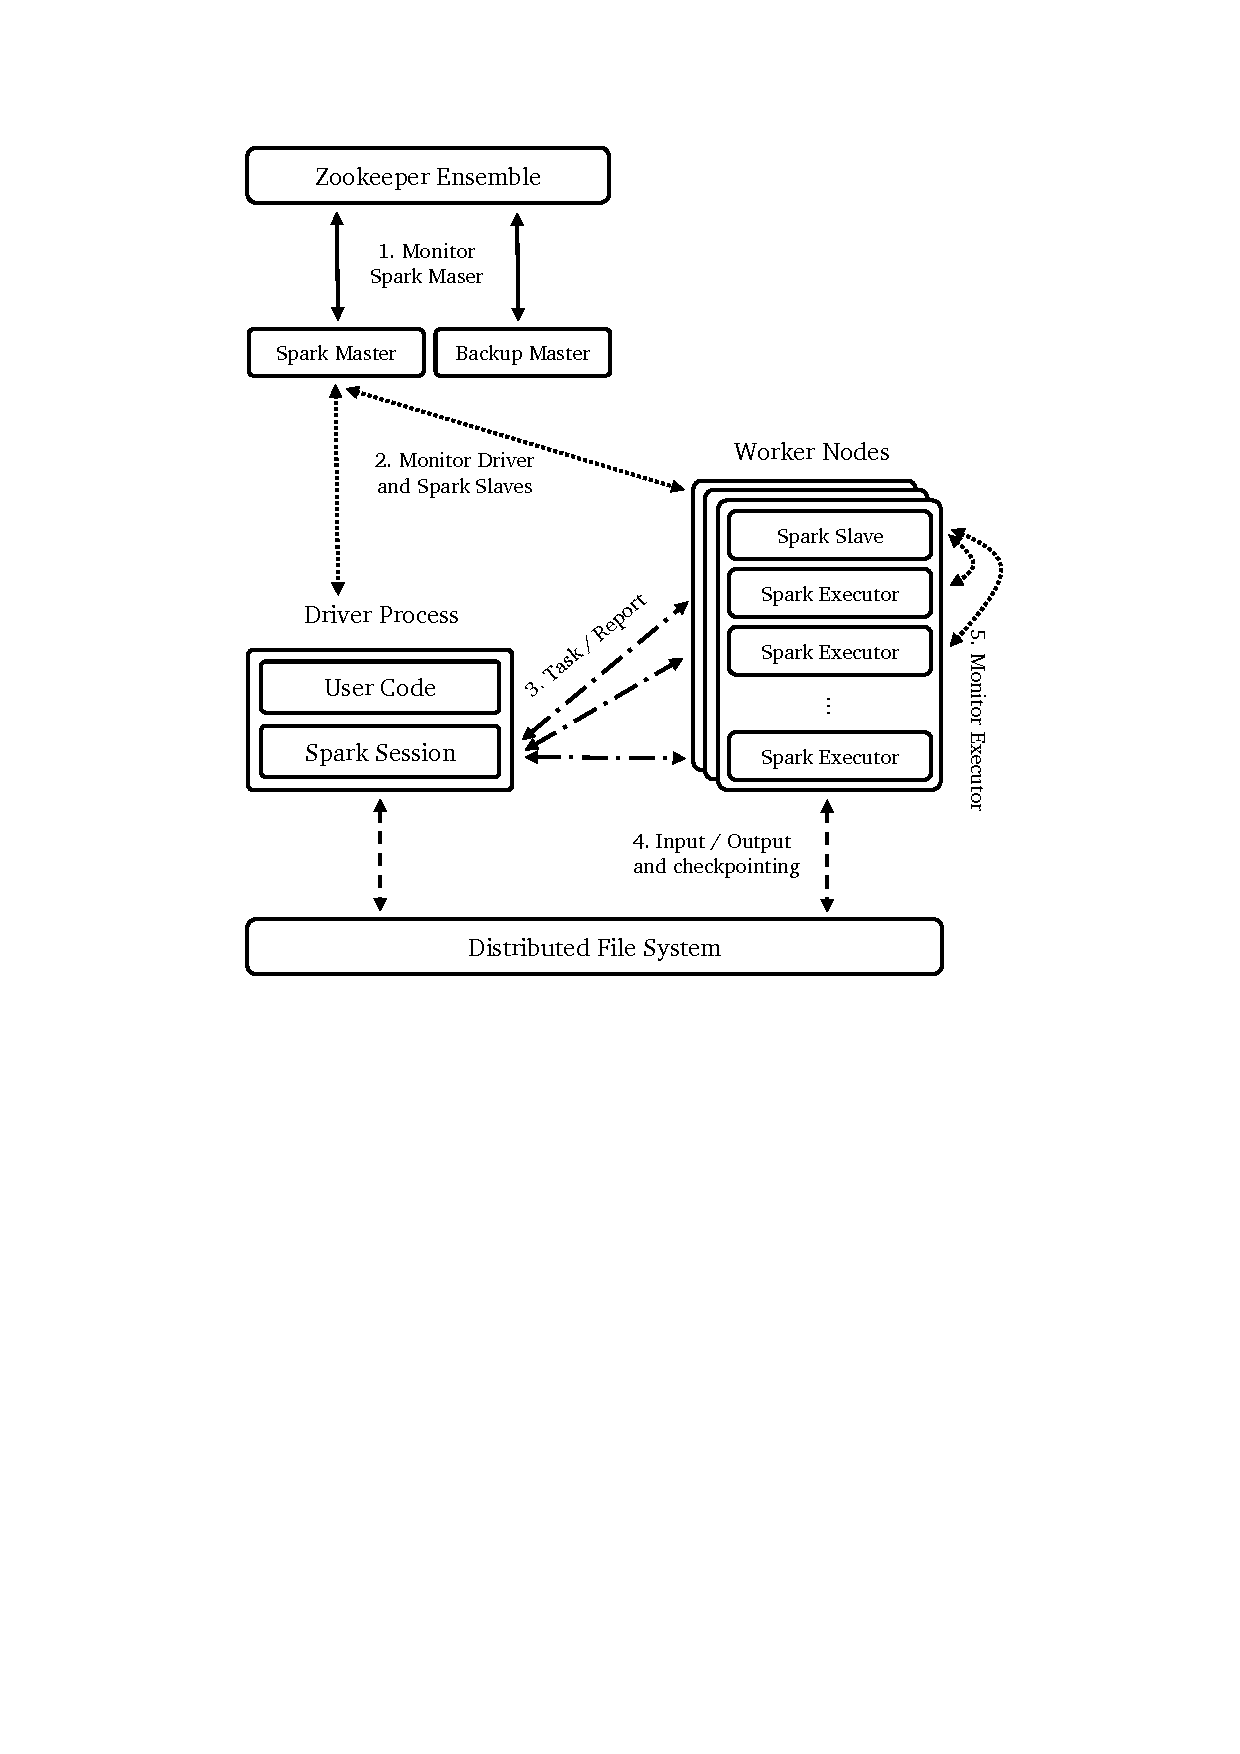
\includegraphics[clip,trim=4cm 13cm 4cm 2.2cm]{spark-full.pdf}
         \caption[Spark Fault-Tolerance Architecture]{Spark Fault-Tolerance Architecture}
         \label{fig:spark-full}
     \end{figure}
\end{description}
\footnotetext{The figure has been partially taken from~\cite{spark-guide}}

\section{Resilient Distributed Datasets}
\label{sp:rdd}

\section{Discretized Streams}
\label{sp:dstream}

\section{Conclusion}
\label{sp:conc}

1. add tasks to spark cluster diagram
spark session is the entry point for spark
2. different modes of operation (mesos yarn standalone mode)
    4. may be add graph
    5. add table for summerization
    
    move all footnote for floats to reference place.

3. RDD
4. checkpointing \& persistence

some examples on how RDD models 

DStreams

replaable streams

DStream paper

further features.
Spark external shuffle service, spark listener framewrk

